\documentclass[tikz,border=5pt]{standalone}
\usepackage[UTF8]{ctex}
\usepackage{amsmath,amssymb}
\usetikzlibrary{arrows.meta,calc,angles,quotes,decorations.pathmorphing,patterns}
\definecolor{ink}{HTML}{243447}\definecolor{blue}{HTML}{2765A2}
\definecolor{green}{HTML}{3F7D5B}\definecolor{red}{HTML}{B74739}
\tikzset{body/.style={draw=ink,thick},vec/.style={draw=blue,thick,-{Latex}},guide/.style={gray!60,dashed},dim/.style={ink,{Latex}-{Latex}},line cap=round,line join=round}
\begin{document}

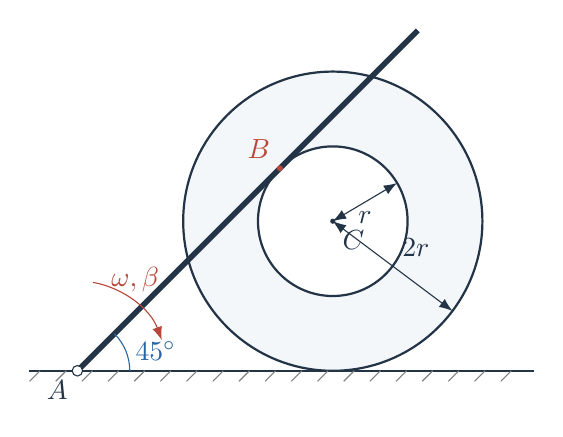
\begin{tikzpicture}[scale=.95]
\coordinate(A)at(0,0);\coordinate(C)at(3.4142,2);\coordinate(B)at(2.7071,2.7071);
\fill[blue!5](C)circle(2);\fill[white](C)circle(1);
\draw[body](C)circle(2);\draw[body](C)circle(1);
\draw[body](-.65,0)--(6.1,0);\foreach\x in{-.5,-.15,...,5.95}\draw[gray](\x,0)--++(-.14,-.14);
\draw[ink,line width=2pt](A)--(4.55,4.55);
\filldraw[fill=white,draw=ink](A)circle(.07)node[text=ink,below left]{$A$};
\fill[ink](C)circle(.035)node[below right]{$C$};
\fill[red](B)circle(.04)node[above left]{$B$};
\draw[dim](C)--++(.86,.51)node[midway,below]{$r$};
\draw[dim](C)--++(1.6,-1.2)node[midway,above right]{$2r$};
\draw[blue](.7,0)arc(0:45:.7)node[pos=.5,right]{$45^\circ$};
\draw[red,-{Latex}](.208378,1.181769)arc(80:20:1.2)node[midway,above]{$\omega,\beta$};
\end{tikzpicture}
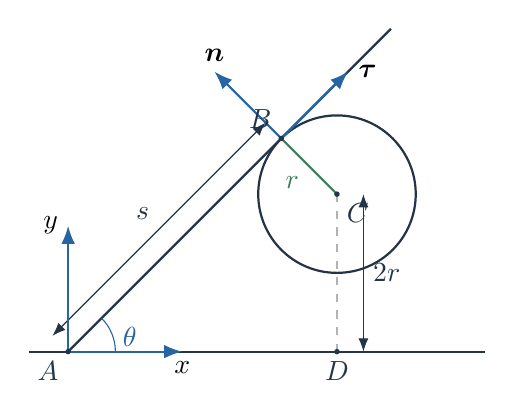
\begin{tikzpicture}
\coordinate(A)at(0,0);\coordinate(C)at(3.4142,2);\coordinate(B)at(2.7071,2.7071);\coordinate(D)at(3.4142,0);
\draw[body](-.5,0)--(5.3,0);\draw[body](A)--(4.1,4.1);
\draw[body](C)circle(1);\draw[guide](C)--(D);
\draw[green,thick](C)--(B)node[midway,below left]{$r$};
\draw[dim](3.75,0)--(3.75,2)node[midway,right]{$2r$};
\draw[dim](-.2,.2)--(2.507,2.907)node[midway,above left]{$s$};
\draw[vec](B)--++(.85,.85)node[right]{$\boldsymbol\tau$};
\draw[vec](B)--++(-.85,.85)node[above]{$\boldsymbol n$};
\draw[vec](A)--(1.45,0)node[below]{$x$};\draw[vec](A)--(0,1.6)node[left]{$y$};
\draw[blue](.6,0)arc(0:45:.6)node[pos=.4,right]{$\theta$};
\foreach\P/\pos in{A/below left,B/above left,C/below right,D/below}\fill[ink](\P)circle(.035)node[\pos]{$\P$};
\end{tikzpicture}
\begin{tikzpicture}
\coordinate(C)at(0,0);\coordinate(B)at(-.7071,.7071);
\draw[body](C)circle(1);\draw[body](-2,-.5858)--(.8,2.2142);
\fill[red](B)circle(.055);\node[left]at(-1.05,.82){$B_c=B_r=B_g$};
\draw[vec](B)--++(.7,-.7)node[right]{$\boldsymbol v_{B_c}=\boldsymbol v_{B_r}$};
\draw[green,-{Latex},thick](B)--++(.7,.7)node[right]{$\dot s\,\boldsymbol\tau$};
\node[align=left,anchor=west]at(1.2,.9){几何位置沿杆迁移\\接触的材料点不断更换};
\fill[ink](C)circle(.035)node[below right]{$C$};
\end{tikzpicture}
\begin{tikzpicture}
\coordinate(C)at(0,0);\coordinate(B)at(-.7071,.7071);
\draw[body](C)circle(1);\draw[guide](-1.4,0)--(1.5,0);
\draw[body](-1.85,-.4358)--(.4,1.8142);
\draw[vec](B)--++(1.8,0)node[above]{$a_C\boldsymbol e_x$};
\draw[green,thick,-{Latex}](B)--++(-.65,-.65)node[below left]{$-r\alpha\boldsymbol\tau$};
\draw[red,thick,-{Latex}](B)--++(1.35,-1.35)node[below right]{$-r\Omega^2\boldsymbol n$};
\fill[ink](B)circle(.04)node[above left]{$B_c$};
\fill[ink](C)circle(.035)node[above right]{$C$};
\node[align=center]at(0,-1.5){示意方向取 $a_C,\alpha>0$};
\end{tikzpicture}
\end{document}
